\documentclass{scrartcl}

\usepackage{lmodern}

\usepackage{tikz}
\usetikzlibrary{automata,positioning}

\begin{document}
  \tableofcontents
  
  \section{Der Reguläre Ausdruck \texttt{|a}}
  
  Initialer Zustand:

  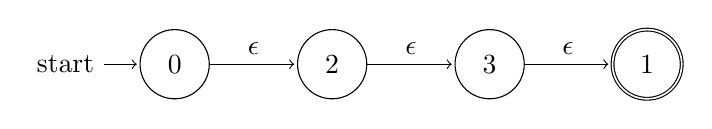
\begin{tikzpicture}[shorten >=1pt,node distance=2cm,on grid,auto]
    \node[state,initial]   (q0)               {$0$};
    \node[state]           (q2) [right=of q0] {$2$};
    \node[state]           (q3) [right=of q2] {$3$};
    \node[state,accepting] (q1) [right=of q3] {$1$};
    
    \path[->] (q0) edge node {$\epsilon$} (q2)
              (q2) edge node {$\epsilon$} (q3)
              (q3) edge node {$\epsilon$} (q1);
  \end{tikzpicture}
  
  Der Reguläre Ausdruck \verb!|a! wird eingefügt in zwei Schritten. Der erste Schritt fügt die linke Regel wischen die Knoten $2$ und $3$ ein. Die linke Regel lautet $\epsilon$, ändert daher nichts am Automaten.
  
  Die zweite Regel lautet \verb|a|. Diese wird zuerst gebaut:
  
  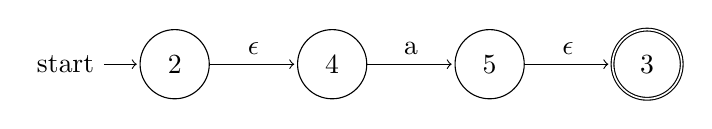
\begin{tikzpicture}[shorten >=1pt,node distance=2cm,on grid,auto]
    \node[state,initial]   (q2)               {$2$};
    \node[state]           (q4) [right=of q2] {$4$};
    \node[state]           (q5) [right=of q4] {$5$};
    \node[state,accepting] (q3) [right=of q5] {$3$};
    
    \path[->] (q2) edge node {$\epsilon$} (q4)
              (q4) edge node {a} (q5)
              (q5) edge node {$\epsilon$} (q3);
  \end{tikzpicture}
  
  Dieser wird jetzt in den ersten Automaten eingehängt:
  
  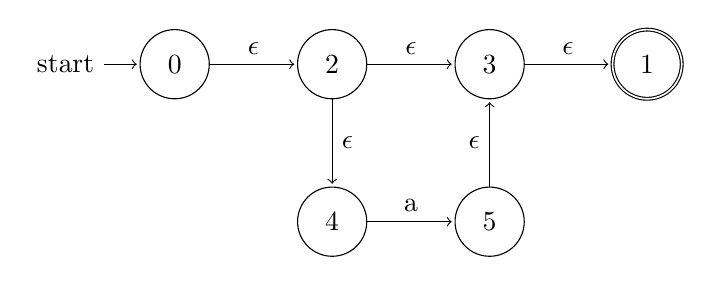
\begin{tikzpicture}[shorten >=1pt,node distance=2cm,on grid,auto]
    \node[state,initial]   (q0)               {$0$};
    \node[state]           (q2) [right=of q0] {$2$};
    \node[state]           (q3) [right=of q2] {$3$};
    \node[state,accepting] (q1) [right=of q3] {$1$};
    
    \path[->] (q0) edge node {$\epsilon$} (q2)
              (q2) edge node {$\epsilon$} (q3)
              (q3) edge node {$\epsilon$} (q1);
              
    % \node[state,initial]   (q2)               {$2$};
    \node[state]           (q4) [below=of q2] {$4$};
    \node[state]           (q5) [right=of q4] {$5$};
    % \node[state,accepting] (q3) [right=of q5] {$3$};
    
    \path[->] (q2) edge node {$\epsilon$} (q4)
              (q4) edge node {a} (q5)
              (q5) edge node {$\epsilon$} (q3);
  \end{tikzpicture}
\end{document}